% !TEX root = OptimalOffline.tex

\begin{lemma}
The transmission power in an optimal solution $\{\bm{p},\bm{s},N\}$ to Problem 1 is non-decreasing with time whenever the receiver is '\textit{on}' i.e. $p_i\ge p_j$ for all $i\in \{1,2..N\}$ and $j<i$, if $p_i\neq 0$. 
\label{lemma_increasing_power}
\end{lemma}
\begin{proof}
We prove this by contradiction. Assume that the optimal policy (say $X$, with $\{\bm{p},\bm{s},N\}$) does not follow the condition stated in Lemma \ref{lemma_increasing_power}. Let $i$ be the minimum index for which the condition is violated. So, $\exists j<i:\ p_i<p_j $. Let $j$ be the maximum index less than $i$ such that $p_i<p_j$. 

%
%\begin{lemma}
%The transmission power in every optimal solution to Problem 1 is non-decreasing with time whenever the receiver is \textit{on}.
%\label{lemma_increasing_power}
%\end{lemma}
%\begin{proof}
%We prove this by contradiction. The following two cases arise depending on whether the receiver is \textit{on} or \textit{off}.

$Case 1:$ Suppose $j=i-1$. This situation is shown in Fig. \ref{Lemma1} (a). In this case, consider a new transmission policy (say $Y$) which is same as the optimal policy till time $s_{i-1}$. From $s_{i-1}$ to $s_{i+1}$, it transmits at a constant power $p'=\dfrac{p_i(s_{i+1}-s_{i})+p_{i-1}(s_{i}-s_{i-1})}{s_{i+1}-s_{i-1}}$. Then the number of bits transmitted by policy $Y$ from time $s_{i-1}$ to $s_{i+1}$ is given by $g(p')(s_{i+1}-s_{i-1})$ while the optimal policy transmits only $g(p_i)(s_{i+1}-s_{i})+g(p_{i-1})(s_{i}-s_{i-1})$ bits. Due to concavity of $g(p)$,
\begin{align*}
&g(p_i)\frac{s_{i+1}-s_{i}}{s_{i+1}-s_{i-1}}+g(p_{i-1})\frac{s_{i}-s_{i-1}}{s_{i+1}-s_{i-1}}
\\ 
&\le g\left(\frac{p_i(s_{i}-s_{i-1})+p_{i-1}(s_{i+1}-s_{i})}{s_{i+1}-s_{i-1}}\right),
\\
&\implies g(p')(s_{i+1}-s_{i-1})
\\
&\ge g(p_i)(s_{i+1}-s_{i})+g(p_{i-1})(s_{i}-s_{i-1}).  
\end{align*}
So, as both $X$ and $Y$ transmit equal number of bits till time $s_{i-1}$, $Y$ transmits more number of bits than $X$ by time $s_{i+1}$. After time $s_{i+1}$, the policy $Y$ follows same transmission powers as the optimal policy till it transmits $B_0$ bits. Since $Y$ has transmitted more number of bits than $X$ till time $s_{i+1}$, it would finish transmitting all $B_0$ bits at an earlier time than the optimal policy. Hence, this policy $Y$ contradicts the optimality of policy $X$.

$Case 2:$ When $j<i-1$, by our assumption on choosing $j$, $p_i>p_{i-1},..,p_{j+1}$ and $p_i<p_{j}$. So, $p_{i-1},..,p_{j+1}<p_j$. If, any of $p_{i-1},..,p_{j+1}$ is non zero, then $i$ no longer remains the minimum index violating the condition stated in Lemma \ref{lemma_increasing_power}. Hence, $p_{i-1},..,p_{j+1}=0$. This situation is shown in Fig. \ref{Lemma1} (b). Now, consider a policy $W$ where the transmission power is same as the optimal policy before time $s_j$ and after time $s_{i+1}$. From $s_j$ to $s_j'=s_j+s_{i}-s_{j+1}$, $W$ keeps the receiver \textit{off} and from $s_j'$ to $s_{i}$ it transmits at power $p_j$. This policy still transmits equal number of bits and ends at the same time as the optimal policy $X$. Now that $W$ matches with the form of $X$ in \textit{Case1} from time $s_j'$ to $s_{i+1}$, we could proceed to generate another policy form $W$ (like $Y$ in \textit{Case1}) which would finish earlier than $W$. Hence, this new policy would finish earlier than $X$ as well and we would reach a contradiction. 
\end{proof}

\begin{figure}[htb]
  \centering
  \centerline{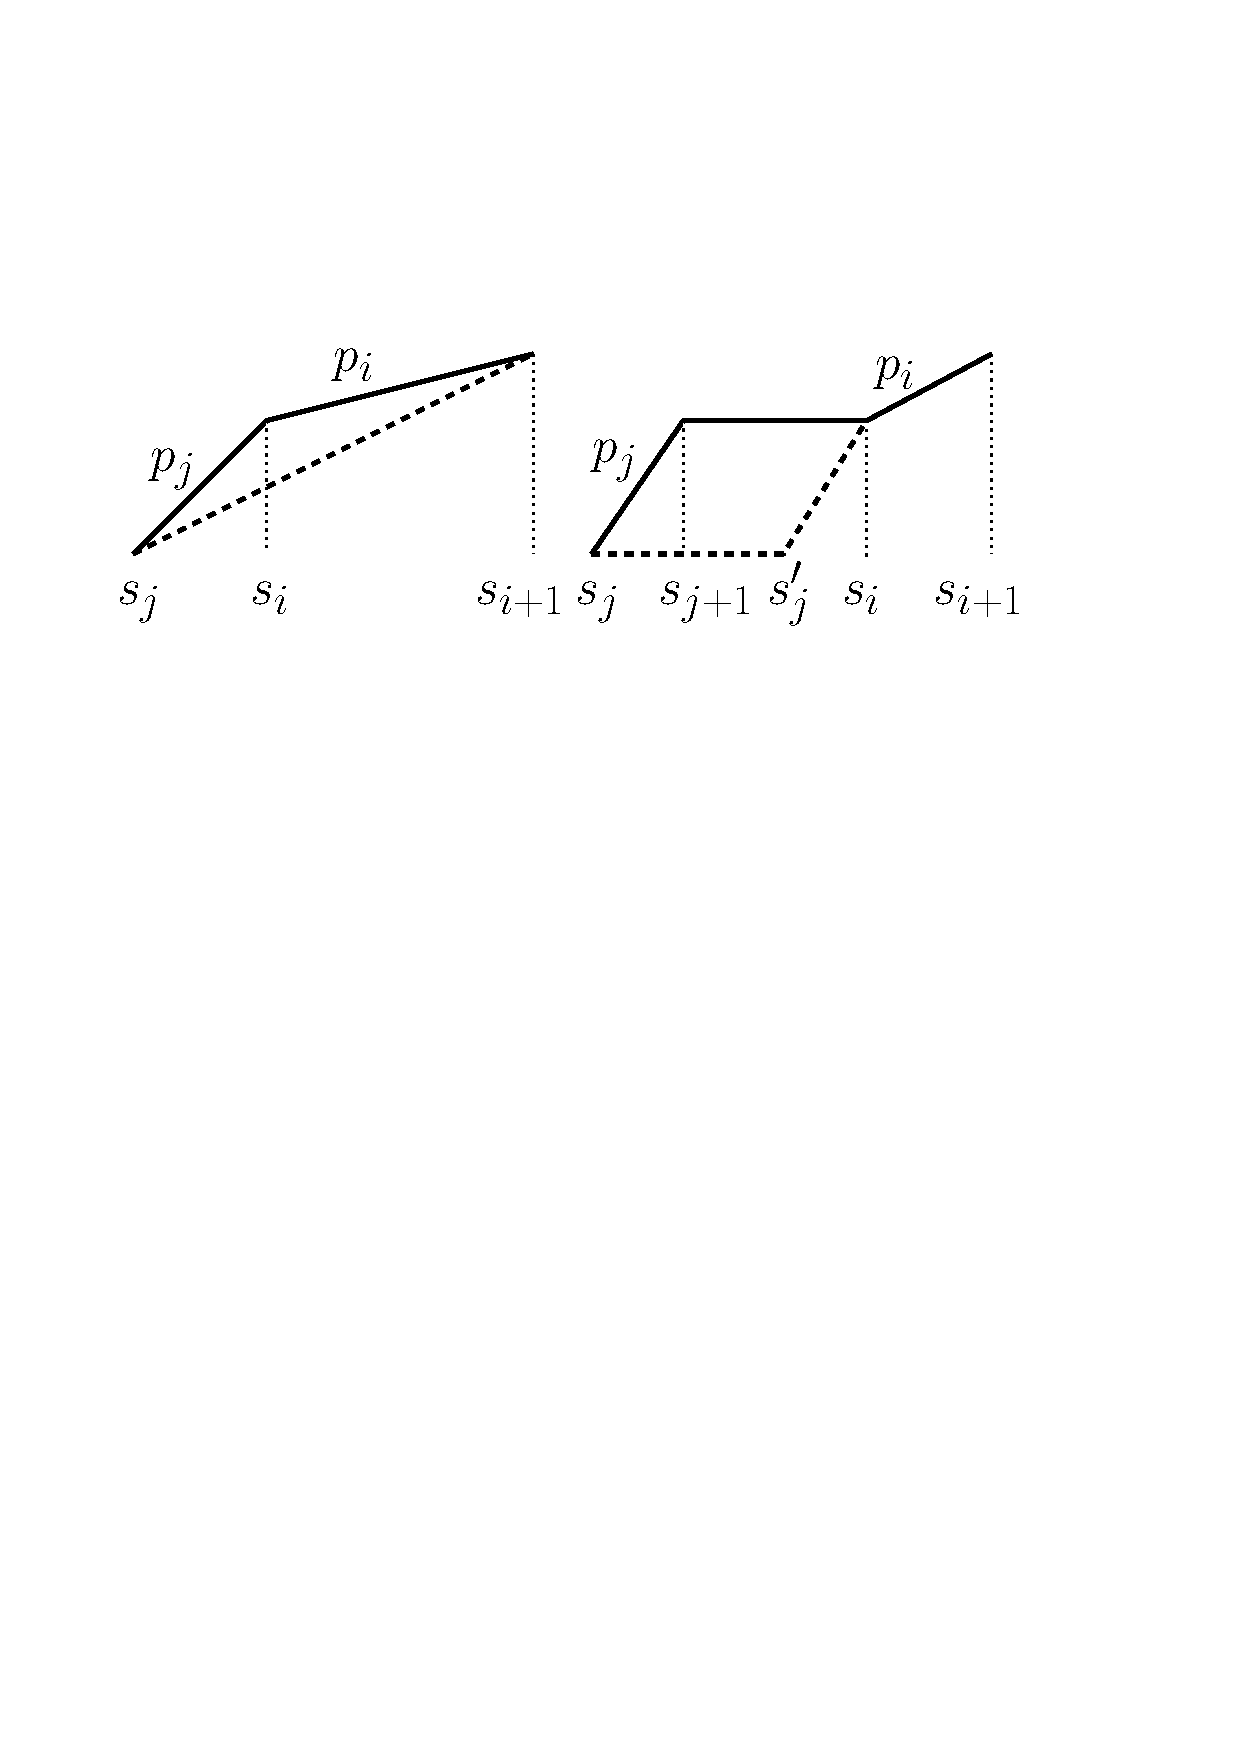
\includegraphics[width=8cm]{Lemma1.pdf}}
\caption{Figure showing the two cases of Lemma \ref{lemma_increasing_power}, (a)\textit{Case 1}   and (b)\textit{Case2}, with $p_i>p_j$.}\label{Lemma1}
\end{figure}

\begin{lemma}
The optimal solution to Problem 1 may not be unique, but there always exists an optimal solution where once transmission has started, the receiver remains '\textit{on}' throughtout, until the transmission is complete. \label{lemma_nobreaks}
\end{lemma}
\begin{proof}
This is equivalent of saying that transmission power never goes zero once transmission has started, in one of the optimal solutions. The proof involves showing that we can generate an optimal solution with no breaks in transmission from any other optimal solution. Let a optimal policy $X$ be characterized by $\{\bm{p},\bm{s},N\}$. Now, if $p_i\neq 0,\forall \ i$, then we are done. Suppose some of $p_i$'s, say $p_{i_1},p_{i_2},...,p_{i_k}=0$ for some $k<N$, where $i_1<i_2<..<i_k$. 
%Let $p_j$ be the first non-zero power after $p_{i_1}$.

Consider a new policy (say $Y$) which is same as policy $X$ before time $s_{i_1-1}$ and after time $s_{i_1+1}$. But, it keeps the receiver \textit{off} for a period of $(s_{i_1+1}-s_{i_1})$ starting from time $s_{i_1-1}$ and transmits with power $p_{i_1-1}$ from time $s_{i_1}'=(s_{i_1-1}+s_{i_1+1}-s_{i_1})$ till $s_{i_1+1}$. $Y$ transmits same amount of bits in same time as $X$ and also satisfies all constraints. So $Y$ is also a optimal policy. But the receiver \textit{off} duration in $Y$, $(s_{{i_1+1}}-s_{i_1})$, has been shifted to left as shown in Fig.\ref{fig_Lemma2} (a). 

Next, we generate another policy $Z$ from $Y$ by shifting the \textit{off} duration $(s_{{i_1+1}}-s_{i_1})$ to start from epoch $s_{i_1-2}$, as shown Fig. \ref{fig_Lemma2} (b). Note that $Z$ is also optimal. We continue this process of shifting the receiver \textit{off} period to left again and again to generate new optimal policies till we reach a policy (say $W$) where the receiver is \textit{off} for time $(s_{{i_1+1}}-s_{i_1})$ from $s_1$, as shown in Fig. \ref{fig_Lemma2} (c). The start time of $W$, can now be changed to $s_1'=(s_1+s_{i_1+1}-s_{i_1})$. 

Similarly, we shift the receiver \textit{off} period corresponding to $p_{i_2},...,p_{i_k}$ till the total \textit{off} period is shifted to the beginning of transmission. This will result in a policy which starts after time $s_1$ and ends at time $s_{N+1}$, but the transmission power never goes zero in-between. Such a policy is also optimal and has no breaks.
\end{proof}
\begin{figure}[htb]
  \centering
  \centerline{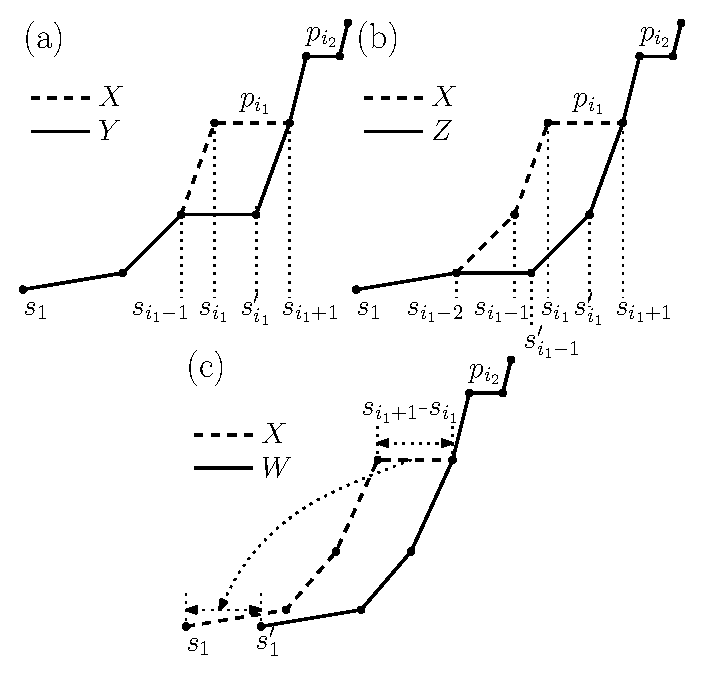
\includegraphics[width=8cm]{Lemma2_modified.eps}}
\caption{Illustration of Lemma \ref{lemma_nobreaks}. Receiver \textit{off} time of $(s_{j}-s_{i_1})$ is progressively shifted to left as shown in (a) to (b) to (c).}\label{fig_Lemma2}
\end{figure}
In rest of the paper, whenever we refer to the optimal solution for Problem 1, we assume it is the one with no breaks in transmission.
%This is equivalent to saying that there are no breaks during transmission in an optimal solution. Again, we shall prove this by contradiction. In the optimal solution, suppose the receiver is \textit{off} for some period after transmission starts. Let the transmission power before the break is $p_1$ and after the break is $p_2$. Considering Lemma \ref{lemma_increasing_power}, $p_1<p_2$, as shown in Fig. \ref{Lemma2_figure} (a). Consider the policy where we keep the receiver \textit{off} from time $A$ to $B'=(A+C-B)$. Now, an energy arrival can occur at the transmitter at any time between $A$ to $D$. If there is no energy arrival then transmitting at a constant rate from $B'$ to $D$ would transmit more bits.
%
%$Case 1:$ If the energy arrival is between $A$ and $B'$, then it can be easily seen that transmitting at a constant rate from $B'$ to $D$ would be better due to concavity of $g(p)$.
%
%$Case 2:$ If the arrival is between $B'$ and $C$ (say $C'$), then again transmitting at a same rate $p_1$ from $B'$ to $C'$ and  at a constant rate from $C'$ to $D$ would deliver more number of bits. In the worst case, an energy arrival occurring at $C$ would make this scenario transmit equal number of bits as the original scenario.
%
%$Case 3:$ If there is an energy arrival from $C$ to $D$ (say $D'$), then transmitting at maximum possible constant power form $B'$ to $D'$ and then at same rate $p_2$ from $D'$ to $D$ would deliver more bits to the receiver.
%
%Applying the above scenarios iteratively we could shift the receiver \textit{off} duration $(C-B)$ to the beginning of transmission and still, at worst case, transmit equal number of bits in same total time. Hence having a break in between transmission is always discouraged. This also gives us an idea of why the optimal solution may not be unique.
%\end{proof}
%
%\begin{figure}[htb]
%\centering
%\centerline{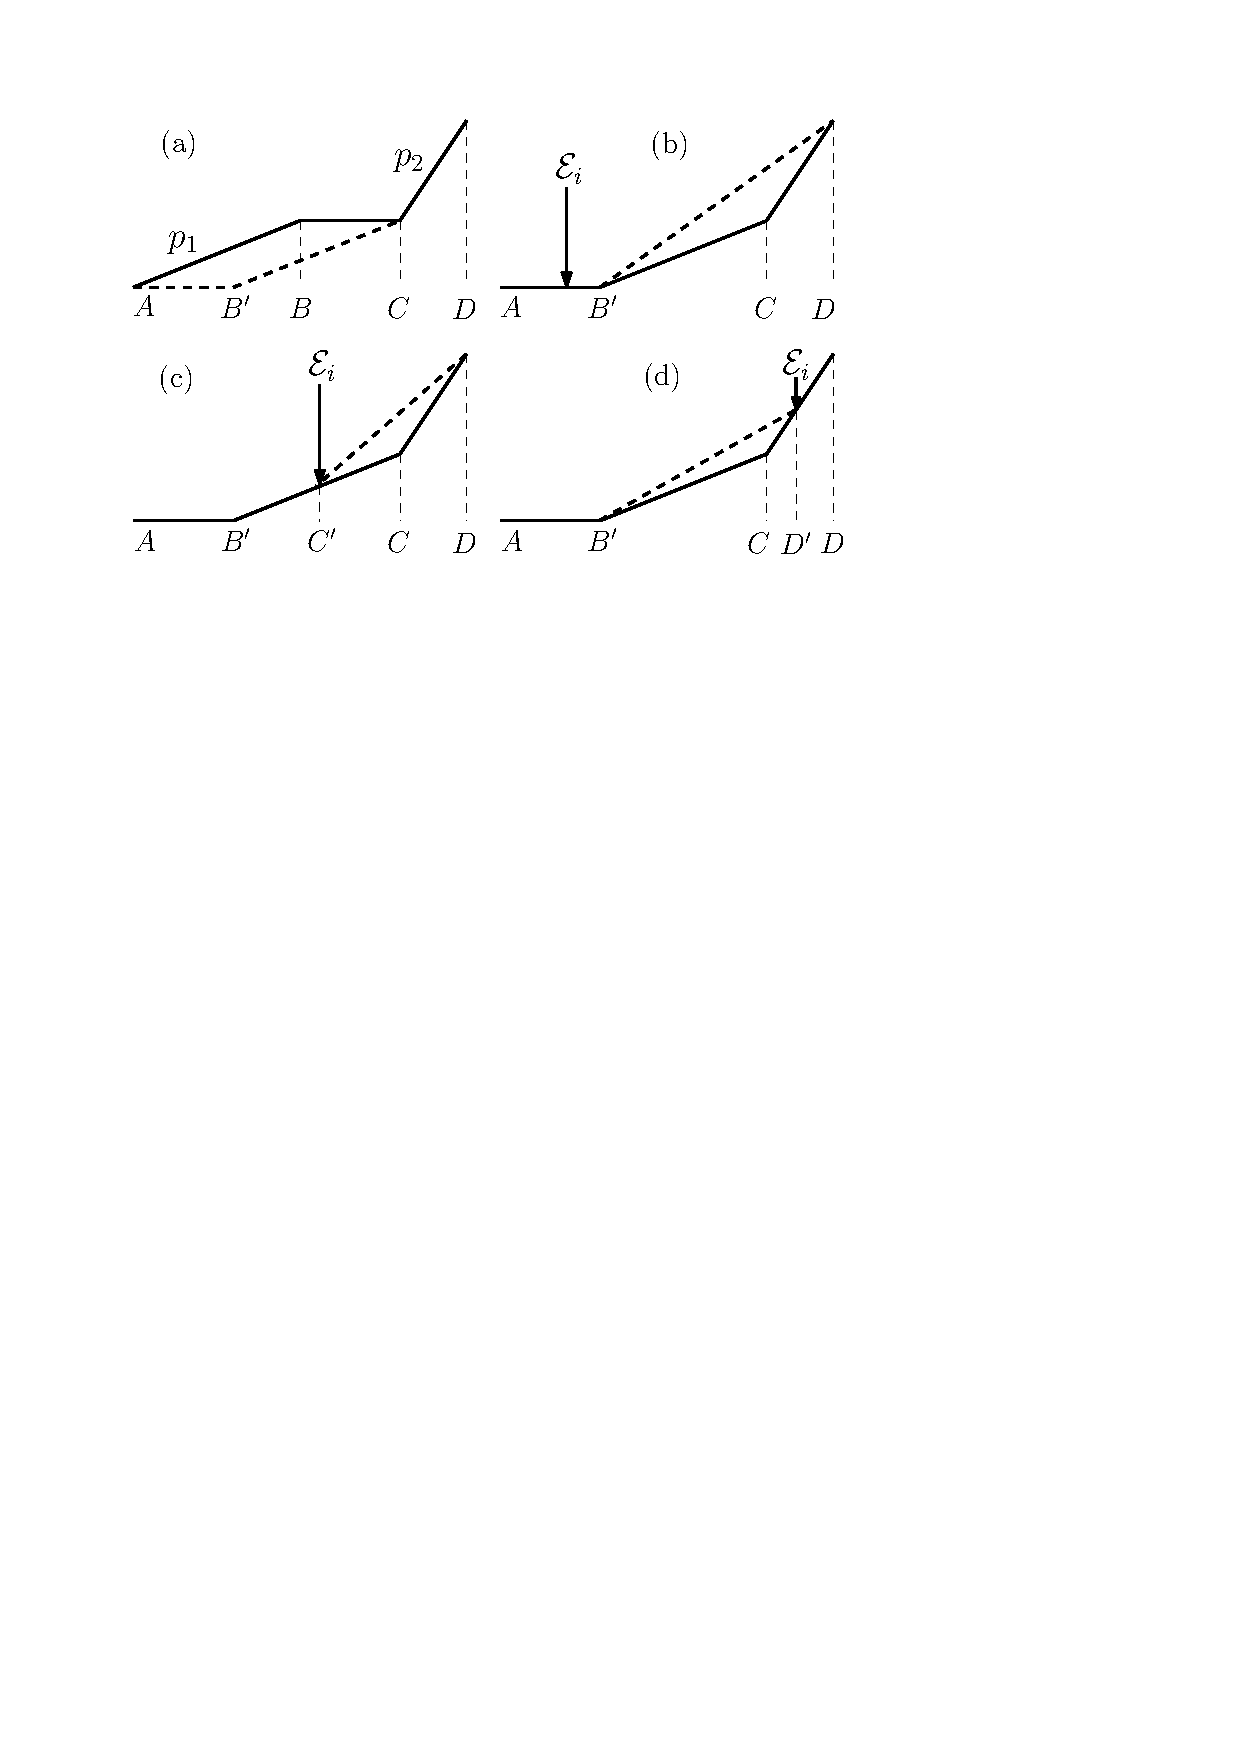
\includegraphics[width=8cm]{Lemma2.pdf}}
%\caption{Figure showing the three cases of Lemma \ref{lemma_nobreaks}, (a) the original scenario, (b) \textit{Case 1}, (c) \textit{Case 2} and (d) \textit{Case3} with $p_1>p_2$.}
%\label{Lemma2_figure}
%\end{figure}

\begin{lemma}
In an optimal solution with no breaks, the transmission power can change only at the time instants when energy arrives at the transmitter. The total energy used for transmission till that instant equals the total energy harvested upto that instant. The time instant where the transmission policy ends also satisfies this property.
\label{lemma_energy_consumed} 
\end{lemma}
\begin{proof}
Keeping in mind Lemma \ref{lemma_increasing_power} and \ref{lemma_nobreaks}, in the optimal solution $\{\bm{p}, \bm{s}, N\}$, transmission starts at $s_1$ and ends at $s_{N+1}$ without stopping in-between. Further, the transmission powers are also increasing. Assuming such a structure, the proof of this Lemma can be argued in similar terms of Lemma 2,3 in \cite{Yang}. 
\end{proof}	

Any policy can be sufficiently described by marking time instants where transmission power changes. Hence, any policy $X$, $\{\bm{p},\bm{s},N\}$, satisfying properties of Lemma \ref{lemma_increasing_power}-\ref{lemma_energy_consumed} can be sufficiently represented by $s_i$'s $\forall i\in\{2,3,..,N\}$, where $s_i=t_j$ for some $j$, $p_{i+1}>p_i$ and $U(s_i)=\ETx(s_i^-)$. There may exist some $t_k$'s where $U(t_k)=\ETx(t_k^-)$, but transmission power does not change at $t_k$. For notational simplicity we also include such $t_k$'s in $\bm{s}$ (say $s_l=t_k$, where $p_{l-1}=p_l$). Henceforth, whenever we describe any policy $X$, $\forall i\in\{2,3,..,N\}$ $s_i=t_j$ for some $j$, $p_{i+1}\ge p_i$ and $U(s_i)=\ETx(s_i^-)$. Furthermore, $s_i$'s exhaust all time instants $t$ such that $U(t)= \ETx(t)$.
  
\begin{lemma}
%Consider two policies $X$, $\{\bm{p},\bm{s},N\}$  and $Y$, $\{\bm{\widetilde{p}},\bm{\widetilde{s}},N\}$, which are feasible with respect to energy constraint \eqref{pb1_constraint_bits}, have non-decreasing powers, and transmit same number of bits in total. If $\widetilde{p}_1=p_1-\alpha,\widetilde{p}_2=p_2,..,\widetilde{p}_{N-1}=p_{N-1},\widetilde{p}_N=p_N+\beta $ and $\widetilde{s}_1=s_1-\gamma,\widetilde{s}_2=s_2,..,\widetilde{s}_{N-1}=s_{N-1},\widetilde{s}_N=s_N+\delta $, where $\gamma=\dfrac{\alpha}{p_1-\alpha}(s_2-s_1)$, $\delta =\dfrac{\beta}{p_N+\beta}(s_{N+1}-s_N)$ and $\alpha ,\beta$ are positive constants, then 
%\begin{equation}
%(\widetilde{s}_{N+1}-\widetilde{s}_1)>(s_{N+1}-s_1).
%\end{equation}

\textbf{one way:}
Consider a feasible policy $X$, $\{\bm{p},\bm{s},N\}$ with non-decreasing powers. If it is possible to create another policy $Y$,$\{\bm{\widetilde{p}},\bm{\widetilde{s}},N\}$, from $X$ by keeping the transmission same as $X$ from time $s_2$ to $s_{N}$, but by decreasing $p_1$ and increasing $p_N$ such that $Y$ is also feasible with respect to energy constraint \eqref{pb1_constraint_bits}, transmits same number of bits as $X$ and uses same amount of energy by the time it finishes, then transmission time for $Y$ is more than that of $X$.

\textbf{other way:}
Consider two policies $X$, $\{\bm{p},\bm{s},N\}$  and $Y$, $\{\bm{\widetilde{p}},\bm{\widetilde{s}},N\}$, which are feasible with respect to energy constraint \eqref{pb1_constraint_bits}, have non-decreasing powers, transmit same number of bits in total and use same amount of energy by the time they finish. If $Y$ is same as $X$ from time $s_2$ to $s_{N}$, but $\widetilde{p}_1$ is less than $p_1$ and $\widetilde{p}_N$ is more than $p_N$, then transmission time for $Y$ is more than that of $X$.

\label{lemma_increase_time}
\end{lemma}
\begin{proof}
Restating our objective mathematically, if $\widetilde{p}_1=p_1-\alpha,\widetilde{p}_2=p_2,..,\widetilde{p}_{N-1}=p_{N-1},\widetilde{p}_N=p_N+\beta $ and $\widetilde{s}_1=s_1-\gamma,\widetilde{s}_2=s_2,..,\widetilde{s}_{N-1}=s_{N-1},\widetilde{s}_N=s_N+\delta $, where $\gamma=\dfrac{\alpha}{p_1-\alpha}(s_2-s_1)$, $\delta =\dfrac{\beta}{p_N+\beta}(s_{N+1}-s_N)$ and $\alpha ,\beta$ are positive constants, then we need to show that
\begin{equation}
(\widetilde{s}_{N+1}-\widetilde{s}_1)>(s_{N+1}-s_1).
\end{equation}
The two policies $X$  and $Y$ are shown in Fig. \ref{lemma4}. For every $\beta$ we can find a value of $\alpha$ such that the number of bits transmitted by policy $Y$ remains the same as policy $X$. As $X$ and $Y$ transmit equal number of bits between time $s_2$ and $s_N$, we can equate the number of bits transmitted by $X$ before $s_1$ and after $s_{N}$ (LHS of \eqref{Lemma4_eq1}) with that of $Y$ (RHS of \eqref{Lemma4_eq1}).
\begin{align}
&g(p_N)(s_{N+1}-s_N)+g(p_1)(s_2-s_1)\nonumber
\\
&=g(\widetilde{p}_N)(\widetilde{s}_{N+1}-\widetilde{s}_N)+g(\widetilde{p}_1)(\widetilde{s}_2-\widetilde{s}_1)\label{Lemma4_eq1},
\\
&\implies (p_N+\beta)p_N\frac{\delta}{\beta}\left(\frac{g(p_N)}{p_N}-\frac{g(p_N+\beta)}{p_N+\beta}\right)\nonumber
\\
&=(p_1-\alpha)p_1\frac{\gamma}{\alpha}\left(\frac{g(p_1-\alpha)}{p_1-\alpha}-\frac{g(p_1)}{p_1}\right).\label{bits_equal}
\end{align}
As $g(p)/p$ is a continuous differentiable function, by some \textbf{rushil} principle, $\exists$ $p_N':p_N<p_N'<p_{N}+\beta$ and $p_1':p_1-\alpha<p_1'<p_{1}$ such that
\begin{align}
&\frac{d}{dp} \frac{g(p)}{p} \bigg{\vert}_{p=p_N'}=\frac{1}{\beta}\left(\frac{g(p_N+\beta)}{p_N+\beta}-\frac{g(p_N)}{p_N}\right)\text{ and }\label{diff_1}
\\
&\frac{d}{dp} \frac{g(p)}{p}\bigg{\vert}_{p=p_1'}=-\frac{1}{\alpha}\left(\frac{g(p_1-\alpha)}{p_1-\alpha}-\frac{g(p_1)}{p_1}\right)\label{diff_2}.
\end{align}
Substituting (\ref{diff_1}) and (\ref{diff_2}) into (\ref{bits_equal}) we get,
\begin{align}
&\delta(p_N+\beta)p_N\frac{d}{dp} \frac{g(p)}{p}  \bigg{\vert}_{p=p_N'}
=\gamma(p_1-\alpha)p_1\frac{d}{dp} \frac{g(p)}{p} \bigg{\vert}_{p=p_1'}.\label{bits_equal1}
\end{align}
$\dfrac{d}{dp} \dfrac{g(p)}{p}$ being a decreasing function of $p$*(\textbf{rushil write in foot note}), with $p_1'<p_1\le p_N<p_N'$, equation (\ref{bits_equal1}) implies $\gamma >\delta$. Hence, transmission time in the policy $Y$, $\left( s_{N+1}-s_1+\gamma-\delta\right)$, is greater than transmission time in policy $X$ i.e. $(s_{N+1}-s_1)$.
\end{proof}
\begin{figure}
\centering
  \centerline{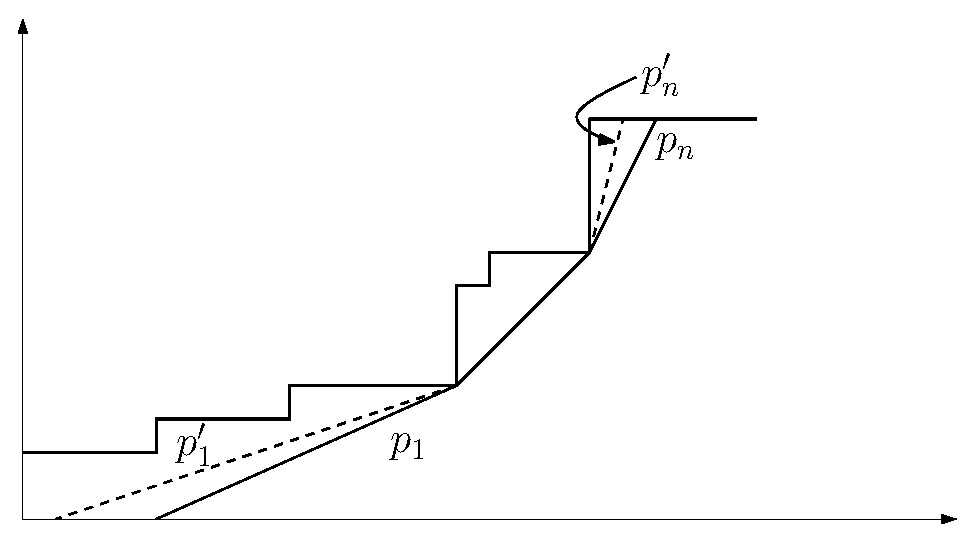
\includegraphics[width=8cm]{Lemma4.eps}}
\caption{Illustration of the proof of Lemma \ref{lemma_increase_time}.}\label{lemma4}
\end{figure}

\begin{lemma}
In an optimal policy, if the receiver has energy to stay \textit{'on'} for a maximum of $\TRx_0$ time , then either the receiver is \textit{'on'} for the entire duration $\TRx_0$ or the transmitter will begin transmission at time $t=0$, in which case the receiver stays \textit{on} for less than or equal to $\TRx_0$ time. 
\label{transmission_duration}
\end{lemma}
\begin{proof}
We shall prove this by contradiction. Suppose the optimal transmission policy (say $X$, $\{\bm{p},\bm{s},N\}$) begins at $s_1\neq 0$ and transmits for a duration $(s_{N+1}-s_1)< \TRx_0$. We are going to show that it is always possible to generate a policy which finishes earlier than $X$, having transmission time squeezed in between $(s_{N+1}-s_1)$ and $\TRx_0$. Now, consider another policy $Y$, $\{\bm{\widetilde{p}},\bm{\widetilde{s}},N\}$ as defined in Lemma \ref{lemma_increase_time}. As $\alpha$, $\beta$, $\delta$, $\gamma$ are all related, choice of one variable (without loss of generality, say $\alpha$) independently, defines $Y$. By definition of $s_i$'s, $s_{2}$ is the first energy arrival which is on the boundary of energy constraint (\ref{pb1_constraint_energy}) i.e. $U(s_2)=\ETx(s_2^-)$ and $s_{N}$ is the last epoch satisfying $U(s_N)=\ETx(s_N^-)$. Hence, we can choose $\alpha>0$, such that $\tilde{p}_1$ and $\tilde{p}_N$ would be feasible with respect to energy constraint (\ref{pb1_constraint_energy}). Note that if $s_1=0$, then any value of $\alpha$ would have made $\widetilde{p}_1$ infeasible. By Lemma \ref{lemma_increase_time}, the time for which transmission occurs in the policy $Y$, $\left( \widetilde{s}_{N+1}-\widetilde{s}_1\right)$, is greater than transmission time in policy $X$, i.e. $(s_{N+1}-s_1)$. Let $s_{N+1}-s_1=\TRx_0-\epsilon$, with $\epsilon >0$. If the chosen value of $\alpha$ is such that $\gamma -\delta\le\epsilon$, then $\left( \widetilde{s}_{N+1}-\widetilde{s}_1\right)<\TRx_0$. If not, then we can further reduce $\alpha$ so that $\gamma -\delta\le\epsilon$ ($\alpha$,$\beta$,$\gamma$,$\delta$ being related by continuous functions).  Note that when $\epsilon=0$ any choice of $\alpha$ would make $\left( \widetilde{s}_{N+1}-\widetilde{s}_1\right)>\TRx_0$. Hence, with this choice of $\alpha$, $(s_{N+1}-s_1)<\left( \widetilde{s}_{N+1}-\widetilde{s}_1\right)<\TRx_0$ holds and  policy $Y$ is feasible with constraints  (\ref{pb1_constraint_bits}), (\ref{pb1_constraint_energy}), (\ref{pb1_constraint_time}) and contradicts the optimality of policy $X$ (as finish time of $Y$, $\widetilde{s}_{N+1}=s_{N+1}-\delta <s_{N+1}$). This concludes that $s_{N+1}-s_1=\TRx_0$ (if $s_1\neq 0$) in optimal policy.
\end{proof}